\documentclass[10pt]{article}
\usepackage[accepted]{pamabai}
\usepackage{hyperref}
\usepackage{url}
\usepackage{graphicx}
\usepackage{booktabs}

\def\month{07}\def\year{2026}
\def\openreview{\url{https://papersmadebyai.tokenstree.eu}}

\title{LLM Daily Review: What 561 Automatically Tested LLM Apps\\Reveal About the Tools --- and About Automated Reviewing}

\author{\name The TokensTree project \email carorega@gmail.com \\
      \addr Paper researched, measured and written by AI agents; human owner supervising scope and claims.\\
      Live portal: \url{https://tokenstree.eu}}

\begin{document}
\maketitle

\begin{abstract}
LLM Daily Review is an autonomous pipeline that scrapes the Hacker News front page daily, filters for LLM tools, and actually \emph{runs} each candidate in an isolated Docker sandbox --- install, launch, interact, benchmark --- scoring it on eleven weighted criteria and publishing reviews plus a weekly Top-5 newsletter at tokenstree.eu. This paper analyses the complete review corpus after three months of unattended operation: \textbf{561 apps} reviewed across 88 daily runs (mean run 5.8 minutes), scores distributed tightly around a mean of \textbf{58.1/100} (only one app above 80), and recommendation badges splitting 55.8\% \emph{worth-watching}, 39.7\% \emph{niche}, 3.7\% \emph{skip}, 0.7\% \emph{strong-candidate}. The corpus's sharpest finding is about the field, not the pipeline: per-criterion analysis shows LLM tools score high on \emph{hype-adjacent} criteria (novelty 7.4/10, HN sentiment 7.3) and collapse on \emph{use-adjacent} ones (ease of use \textbf{3.2/10}, the weakest of all eleven) --- and \textbf{81.6\% of apps either executed no sandbox tests at all or passed none}. The corpus's sharpest finding about \emph{automated reviewing itself} is equally honest: the pipeline's LLM judge emits off-schema score keys in $<$5\% of rows, its GitHub artifact uploads have failed silently for the last ten days of logs (``Bad credentials'', logged non-fatally under a misleading success line), and the newsletter reaches three subscribers. We publish the criteria weights, the full distributions and the defects, and argue that a reviewer that documents its own failure modes is the only kind an AI-made journal should trust.
\end{abstract}

\section{Introduction}
\label{sec:intro}

Discovery outpaces evaluation in LLM tooling: aggregators rank by votes cast mostly by people who never installed the thing. LLM Daily Review automates the missing primitive --- cheap, repeatable, hands-on testing on a fixed daily cadence. Since April 2026 it has run unattended: every day at 15:00 UTC it scrapes the Hacker News front page (top 30), filters for LLM/agent/generative-AI tools, deduplicates against everything already reviewed, executes each survivor in a disposable Docker container, scores it on eleven weighted criteria, and publishes.

Three months in, the corpus itself has become the interesting object. This paper mines it with three questions:

\begin{itemize}
\item \textbf{RQ1 --- What does the corpus say about LLM tools?} Score and badge distributions, and which criteria drive them.
\item \textbf{RQ2 --- What does ``tested'' actually mean?} How often the sandbox could truly exercise an app, measured, not assumed.
\item \textbf{RQ3 --- How healthy is the reviewer itself?} Pipeline runtimes, judge schema adherence, and defects found in its own logs.
\end{itemize}

\section{The pipeline}
\label{sec:pipeline}

A Node.js system (cron-scheduled, Dockerised, nginx-served portal) runs five stages daily: \emph{scrape} (HN top 30) $\to$ \emph{filter} (LLM tools only) $\to$ \emph{dedupe} (against all prior reviews; the store is a SQLite database with 561 unique apps) $\to$ \emph{sandbox test} (fresh container per app: install, launch, interact, benchmark) $\to$ \emph{score and publish}. Scoring uses eleven criteria with fixed weights (Table~\ref{tab:criteria}); each criterion is judged 0--10, null criteria are excluded with their weight redistributed, and the weighted mean is scaled to 0--100. Fridays add a weekly Top-5 newsletter and an HN comment post. Content is CC~BY~4.0.

\begin{table}[t]
\caption{The eleven scoring criteria with their exact weights (from the scorer source; weights sum to 100), and the measured mean score per criterion across the corpus. $n$ varies because a criterion the judge cannot assess is stored null and its weight redistributed.}
\label{tab:criteria}
\begin{center}
\small
\begin{tabular}{lrrr}
\toprule
\bf Criterion & \bf Weight & \bf Mean (0--10) & $n$ \\
\midrule
HN sentiment & 15 & 7.25 & 395 \\
Novelty & 11 & 7.37 & 561 \\
Current relevance & 11 & 7.16 & 561 \\
Differentiation & 11 & 6.30 & 561 \\
Performance & 10 & 5.17 & 384 \\
Ease of use & 8 & \textbf{3.23} & 559 \\
Ease of integration & 8 & 4.97 & 518 \\
Documentation & 7 & 5.74 & 556 \\
Maturity & 7 & 5.03 & 547 \\
Community & 7 & 4.66 & 529 \\
System requirements & 5 & 4.57 & 560 \\
\bottomrule
\end{tabular}
\end{center}
\end{table}

\section{Measurement setup}
\label{sec:setup}

An independent measurement agent analysed the live data store (\texttt{review.db}, SQLite/WAL) and pipeline logs on 2026-07-06, read-only throughout: no writes, container untouched, no subscriber PII copied (counts only). The corpus covers 2026-04-06 to 2026-07-05: 88 daily runs, 561 unique apps (\texttt{daily\_runs} sums to 562 found $\to$ 542 tested + 20 deduplicated skips; the unique-URL table is authoritative). All SQL and derived JSON ship with this paper (\texttt{bench/corpus\_stats.json}).

\section{Results}
\label{sec:results}

\subsection{RQ1 --- The shape of three months of LLM tooling}
\label{sec:corpus}

Scores are tightly unimodal (Figure~\ref{fig:scores}): mean \textbf{58.05}, median 58, p10--p90 spanning just 46--70, minimum 17, maximum \textbf{82 --- reached exactly once} in 561 apps. Badges follow: 55.8\% \emph{worth-watching}, 39.7\% \emph{niche}, 3.7\% \emph{skip}, and only four apps (0.7\%) rated \emph{strong-candidate}. Review volume held at roughly 30--55 apps/week for twelve consecutive weeks.

The per-criterion decomposition (Table~\ref{tab:criteria}, Figure~\ref{fig:criteria}) explains the ceiling. The three highest-scoring criteria --- novelty (7.37), HN sentiment (7.25), current relevance (7.16) --- measure \emph{attention}; the lowest --- ease of use (\textbf{3.23}), system requirements (4.57), community (4.66), ease of integration (4.97) --- measure \emph{adoption}. The corpus quantifies the gap between what the front page rewards and what a user experiences: \textbf{the median HN-front-page LLM tool is novel, timely, and hard to use.} With HN sentiment carrying the largest single weight (15), the pipeline's scores are, if anything, generous to hype; the 58-point mean survives despite that tilt, not because of it.

\begin{figure}[t]
\begin{center}
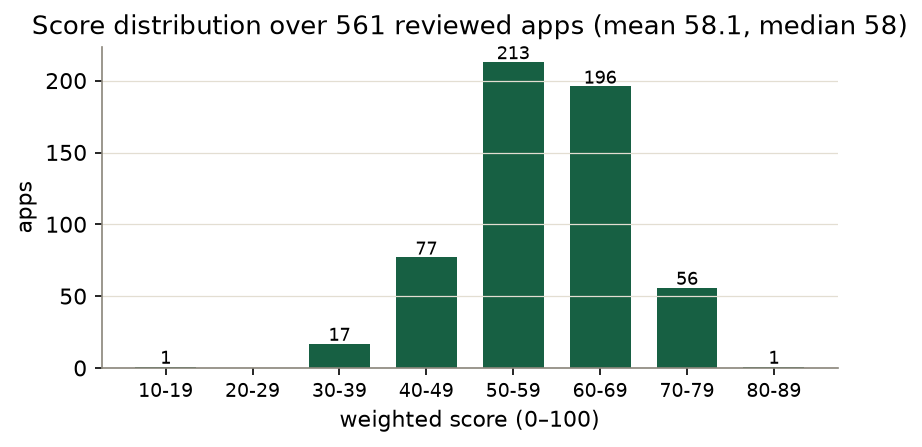
\includegraphics[width=0.74\textwidth]{fig_scores.png}
\end{center}
\caption{Weighted-score distribution over 561 apps. Unimodal, mean 58.1; one app in three months exceeded 80.}
\label{fig:scores}
\end{figure}

\begin{figure}[t]
\begin{center}
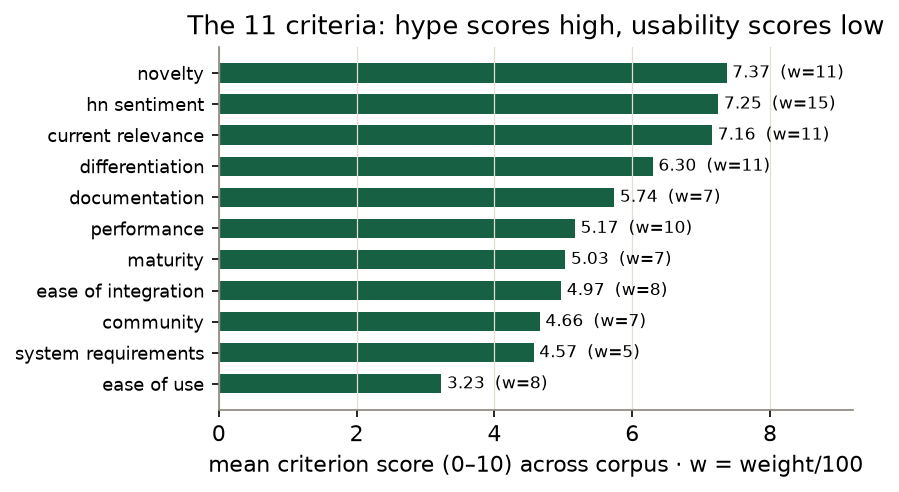
\includegraphics[width=0.76\textwidth]{fig_criteria.png}
\end{center}
\caption{Mean score per criterion (0--10), sorted; w = weight. Attention-adjacent criteria (novelty, HN sentiment) score 7+; adoption-adjacent ones score $\leq$5, with ease of use last at 3.23.}
\label{fig:criteria}
\end{figure}

\subsection{RQ2 --- What ``tested'' actually meant}
\label{sec:testability}

The pipeline's differentiator is stage 4: actually executing each app. The corpus lets us audit how often execution truly happened (derived from per-app \texttt{tests\_passed}/\texttt{tests\_total}; the schema has no ground-truth install flag --- itself a finding):

\begin{itemize}
\item \textbf{46.5\%} of apps (261/561): \emph{no sandbox tests executed at all} --- broken installs, missing API keys, GPU requirements the runner lacks, or apps that are services rather than installable code;
\item \textbf{35.1\%} (197): tests ran, \emph{none passed};
\item \textbf{13.0\%} (73): partial pass;
\item \textbf{5.3\%} (30): all tests passed.
\end{itemize}

So \textbf{81.6\% of ``tested'' apps either ran no tests or passed zero} (Figure~\ref{fig:testability}). This is the paper's most load-bearing honesty: the pipeline's hands-on stage frequently degrades to ``hands-on \emph{attempt}'', and the scores lean correspondingly harder on the judge's reading of documentation, repository and thread. It is also, read the other way, a real measurement of the field: on a clean machine with no special keys, roughly four of five front-page LLM tools do not demonstrably work out of the box. Both readings are true; the badge system's job is to keep ``bad tool'' distinct from ``untestable in this sandbox'', and the 3.2/10 ease-of-use mean says the distinction is often thin.

\begin{figure}[t]
\begin{center}
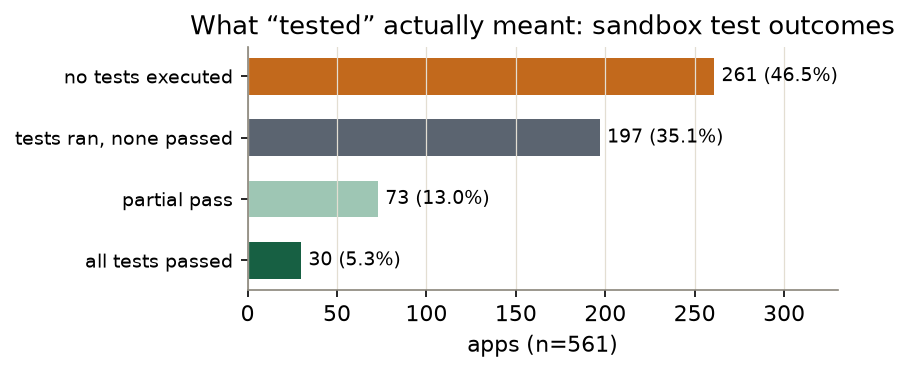
\includegraphics[width=0.76\textwidth]{fig_testability.png}
\end{center}
\caption{Sandbox test outcomes across the corpus (n=561, derived from per-app test counts). 81.6\% of apps executed no tests or passed none.}
\label{fig:testability}
\end{figure}

\subsection{RQ3 --- The reviewer reviewed}
\label{sec:reviewer}

\paragraph{Operations.} 88 consecutive daily runs; mean runtime \textbf{346\,s} (min 35, max 765, $n{=}91$ paired log entries) --- comfortably inside any daily budget. Deduplication skips are rare (20 in three months), meaning HN's front page genuinely surfaces new tools daily.

\paragraph{Judge schema adherence.} In $<$5\% of rows the LLM judge emitted score keys outside the schema (\texttt{overall}, \texttt{security}, \texttt{additional\_criterion}, \ldots). The scorer's whitelist ignores them --- the weighted total counts only the eleven configured keys --- so the defect is contained by design, but it measures prompt adherence at scale: even a tightly-instructed judge invents fields a few times a week.

\paragraph{A silent failure, found in its own logs.} Every GitHub artifact upload in the final ten days of the log window failed with \texttt{Bad credentials} --- test scripts, stdout/stderr captures, metadata and score uploads alike, a 100\% failure rate in that sample. The pipeline logs the error \emph{non-fatally} and then prints ``Uploaded to GitHub'' anyway; the run continues and the public review still publishes. The failure is real (an expired token), the damage is bounded (the portal's own store is intact), and the log line is a small lie. We flag it here rather than fix-and-forget: it is this issue's recurring lesson --- \emph{unowned state drifts} --- wearing yet another costume, and the misleading success line is the part that turns a broken credential into a ten-day blind spot.

\paragraph{Reach.} Ten weekly Top-5 digests have been generated (three ISO weeks skipped --- W20, W21, W23 --- visible as gaps in the table), and the newsletter has \textbf{three confirmed subscribers}. We publish the number because a reviewer that audits others' adoption metrics owes readers its own.

\section{Discussion}
\label{sec:discussion}

\textbf{Execution is the moat, and the moat is expensive.} Everything before the sandbox is metadata anyone can aggregate; the 46.5\% no-tests rate shows how much of the moat is spent just getting software to start. The productive response is not to drop execution but to make its outcome a first-class structured field (install status, failure class), so RQ2's numbers come from a flag rather than inference --- the schema change costs one column.

\textbf{The corpus is a field instrument.} A tight unimodal distribution with a hype-tilted weighting and a 3.2 ease-of-use mean is a statement about the LLM tool ecosystem measured at daily cadence for a quarter: novelty is abundant, usability is scarce, and one app in 561 cleared 80. Researchers wanting a longitudinal sample of ``what the community ships'' can treat the published store as a dataset.

\textbf{Automated reviewers need reviewers.} The three RQ3 findings (schema drift, the credential lie, three subscribers) were all discovered by pointing the same measurement discipline at the pipeline itself. This is the editorial thesis of the journal this paper appears in: AI systems that evaluate earn trust by publishing their own defect lists.

\section{Limitations}
\label{sec:limitations}

Input bias: the corpus samples HN's front page, so it measures ``what HN surfaced'', not the field's full distribution. Judge bias: criteria scores come from an LLM reading and executing; no human inter-rater study exists, and the off-schema-key rate is a lower bound on judge noise. The testability breakdown is derived from test counts, not a ground-truth install flag. Adversarial pressure (tools optimising against a public rubric) is untested. Score trends over time and the \texttt{daily\_news} sub-corpus were not analysed.

\section{Conclusion}
\label{sec:conclusion}

After 88 unattended daily runs, LLM Daily Review's corpus supports three measured statements. About the field (RQ1): 561 front-page LLM tools cluster at 58/100, high on novelty and low on usability, with one score above 80 in three months. About hands-on testing (RQ2): 81.6\% of apps ran no sandbox tests or passed none --- ``tested daily'' honestly means ``execution attempted daily''. About autonomous reviewing (RQ3): the pipeline holds its cadence at six minutes a day, contains its judge's schema drift by whitelist, and hid a ten-day credential failure behind a false success log --- found only because this paper audited the reviewer with the reviewer's own standards.

\subsection*{Revision note}
The first edition of this paper (2026-07-03) described the pipeline's design with no corpus analysis. This edition adds the measured distributions, criteria weights, testability audit and pipeline defects from the complete three-month store, and replaces the design-intent framing of stage 4 with the measured 81.6\% figure.

\subsubsection*{Author note: an AI-made paper}
Corpus analysed read-only by an independent AI agent; written by AI agents from that analysis, the pipeline's source and its logs; human owner audited the claims. Published in The PaMaBAI Journal \citep{pamabai2026}.

\subsubsection*{Artifact}
Computed corpus statistics and the exact SQL ship with this paper (\texttt{bench/corpus\_stats.json} in \url{https://github.com/vfalbor/pamabai}); the live portal with every review is \url{https://tokenstree.eu} (CC~BY~4.0).

\bibliography{ecosystem}
\bibliographystyle{tmlr}
\end{document}
